%# -*- coding: utf-8-unix -*-
%%==================================================
%% chapter02.tex for SJTU Master Thesis
%% related work
%%==================================================
%\bibliographystyle{sjtu2}%[此处用于每章都生产参考文献]

\chapter{相关工作}
\label{chap:related}


\section{国内外研究现状}
\label{sec:situation}

\subsection{相似轨迹查询方法}
\label{subsec:situation-methods}
轨迹数据挖掘中,相似轨迹数据查询国内外有着较为丰富的研究成果。最初的相似轨迹查询通过首先对一段序列数据进行离散傅里叶变化(Discrete Fourier Transform),根据帕塞瓦尔定理在$O(nlogn)$实现时间复杂度内将轨迹做近似匹配得到相似轨迹\cite{agrawal1993efficient}。在此基础上,通过离散小波变换(Discrete Wavalet Transformation)在降低查询维度上的相似轨迹匹配得以实现\cite{chan1999efficient}。为了能够比较不同单位长度轨迹之间相似性,Chan和Fu通过动态时间规划(Dynamic Time Warping)的技术来来最小化轨迹序列之间的距离以完成相似轨迹查找\cite{bernad1996finding},虽然这一方法在处理噪音点上具有鲁棒性,但操作相对于目前算法而言过于繁琐。

较早通过欧式距离作为关键字索引轨迹的方法\cite{yanagisawa2003shape}只能引用于在时间和空间上具有相同间隔性的轨迹数据。之后Cai和Ng提出基于切比雪夫多项式(Chebyshev polynomials)的轨迹索引和近似方法来实现相似轨迹匹配\cite{cai2004indexing}。但上述方法都需要保证轨迹具有相同的长度,即相同数目的轨迹点。

Vlachos等人用一种距离度量来转义和变换轨迹以找到相似轨迹\cite{vlachos2004rotation},结合动态时间规划技术,将所有轨迹变化到一个不可转变的空间再计算两个轨迹之间的相似性。Sakurai等在动态时间规划的基础上,结合剪枝算法用下界变量来加快动态时间规划的相似轨迹查询算法\cite{sakurai2005ftw}。Lin和Su提出与时间无关、针对移动轨迹的相似搜索算法重点比较两个移动在空间上的相似性并实现查询,并在他们的实验中证明了该方法优于基于动态空间规划的相似轨迹查询。

一种名为Fr\'{e}chet\cite{alt1995computing}距离的相似度方程在相似轨迹查询中有着比较普遍的应用。假设一个人和一只狗用一根绳子连接,从起始点各自沿着一条路径行走到终点,并允许他们以不同的速度前进但不允许往回走。直观理解而言,Fr\'{e}chet距离就是狗绳距离:人和狗各自在走完各自路径所需要的最短的狗绳长度。两个各有$m$和$n$个离散点组成的轨迹之前的Fr\'{e}chet距离可以在$O(mnlog(m+n))$时间复杂度内计算,对于离散型的轨迹点,\cite{alt1995computing}称之为离散Fr\'{e}chet距离,可以通过动态规划算法在$O(mn)$时间复杂度内计算。之后Agarwal等人\cite{agarwal2014computing}也提出并验证了离散Fr\'{e}chet距离在次二次时间复杂度内的计算方法。

但该算法对于两条交错轨迹的相似度计算应用上存在一些需要提高的地方。对于给定的一对轨迹$T1$和$T2$,可能会有大量的潜在轨迹点对能够产生理论上合理的Fr\'{e}chet距离。因此通过最小化Fr\'{e}chet距离来表示轨迹之间的相似度并不一定能够满足之后的需求。为了解决这个问题,研究人员通过用将Fr\'{e}chet距离平均化而不是最小化来表示轨迹之间的相似度。这个思路的具体时间基于目前比较流行的动态时间规整(Dynamic Time Warping)技术。动态时间规整技术最初是提出并应用是在对声音信号的匹配上\cite{rabiner1993fundamentals},在相似轨迹查询这一领域,动态时间规整技术可以较有效地查询采样率不同的相似轨迹。因为这一技术通过对两条轨迹之前所有点都进行一一匹配,结果准确性会因为一些噪音点或者轨迹点偏差而受到影响。由于测量造成的误差在目前轨迹处理技术中还缺乏准确有效地预处理技术。针对这种潜在的轨迹数据误差,最长公共子序列算法\cite{vlachos2002discovering}等算法得以提出以在相似轨迹查询中对误差数据具有较好的鲁棒性。

最长公共子序列算法(Longest Common Subsequence)算法在字符串中应用也在拓展于相似轨迹查询中。最长公共子序列问题的本质描述两字符串之间的相似度,在解决问题过程中允许对两个字符串进行扩展。算法本身允许其中的某些字符不匹配,这也匹配在相似轨迹查询中允许某些点不匹配。因此最长公共子序列可高效解决噪音点问题和允许轨迹间隔不同。Vlachos等人在最长公共子序列的基础上,提出两种针对时间变化与转移的相似度方程\cite{vlachos2002discovering},对于相似的子轨迹在计算中基于较大权值,并利用了高效的空间索引结构。但这一算法局需要轨迹点的采样率高度一致性。

随后,一种名为EDR\cite{chen2005robust}(Edit Distance On Real Sequences)的方法被提出。这个方法基于对距离的修改,通过三种剪枝策略以降低轨迹数据和查询数据之间的距离计算代价,在处理噪音点方面鲁棒性强于动态时间规划和最长公共子序列。但准确性上缺乏保证且对于不同采样率的轨迹处理性能较差。类似该工作,Sayan Ranu等人提出了EDwP\cite{ranu2015indexing}(Edit Distance with Projections)的相似轨迹查询方法。其主要思路在于对轨迹之间相互投影,使得经过投影部分的轨迹序列在地理形状上和时序上保持一致性或相似性。在投影过程中对已投影的轨迹用自定义的一种名为TrajTree的所以结构进行存储,其中越靠近根节点的轨迹数据表示具有越多一致或相似部分的轨迹。作者也通过实验验证该算法对噪音点处理上的强鲁棒性和TrajTree数据结构在进行k最近邻查询时的高效性,不过该方法过程对轨迹相似度的查询中对时间间隔较大的轨迹数据查询性能相对较差。



在此之后,针对时序相似度获取的ERP(Edit distance with Real Penalty)\cite{chen2004marriage}算法被提出。这一算法被认为是L1范式和距离修改方程的较好结合算法:L1范式应用在相似度距离方程中而用距离修改方程解决时间偏移问题。由于ERP算法是基于距离修改方程,该算法可以在k最近邻查询剪枝过程中处理三角不等式带来的相似度问题。而在轨迹存储上,ERP算法选择了$B^{+}$树来存储轨迹数据以在该算法中减少存储需求和节约可能的I/O开销。这种结合这可以看成是GEMINI (GEnome MINIng) 对时序数据索引的拓展工作。


DISSIM\cite{frentzos2007index}和MA(model-driven assignment)\cite{sankararaman2013model}等等针对相似轨迹查询的算法也逐步提出且各具优势,不过他们在时间偏移、采样速率和距离阈值限制上也都有着不足。

另一方面,在生物计算方面的序列校准领域的研究技术,例如找到DNA或蛋白质的序列相似度,也通过在某些情况下使用于相似轨迹的查询领域。书\cite{durbin1998biological}中提及的通过建立模型来分析生物序列的方法,被拓展为对两条轨迹序列的校准。这一方法在处理相似轨迹时会有较好的应用性能。但是对于采样率不同的轨迹,基于方法\cite{durbin1998biological}的相似轨迹处理会使得轨迹间原本相似的部分由于算法建模中一一对应原则导致被视作不相似的。


\subsection{相似度方程比较}
\label{subsec:situation-sim-fun-compare}


图\ref{fig:existing-sim-funs}对上述部分算法中涉及的相似度方程给出定义,以比较其中不同。这些方程根据自身特点与优势应用于不同的场景中\cite{morse2007efficient},包括欧氏距离方程(Euclidean Distance),动态时间规整(Dynamic Time Warping),最长公共子序列算法(Longest Common Subsequence),基于编辑代价的方法(Edit Distance With Real Penalty)和基于序列编辑的距离方法 (Edit Distance on Real Sequences)。动态时间规整(DTW)方法在比较轨迹之间相似性的过程中采用了时间偏移(time-shifting)来使得轨迹中的一些点可以尽可能多地重复出现以实现最好效果的校准。但这种方法在原有轨迹数据点出现误差(或称为噪声点)的时候会影响比较的准确性因为所有的点都需要被匹配。相比如动态时间规整方法(DTW),最长公共子序列(LCSS)选择忽略某些点以避免对他们的重排序过程,从结果上而言这种方法舍弃了偏离采样的误差点以提高了准确性,但需要人为预定距离阈值以判断什么数据属于误差点。基于编辑代价的距离方法(EDR)与LCSS方法类似,他们最初提出是为了解决字符串匹配问题,在轨迹数据匹配这一方面他们均采用一个阈值参数来判断两个点是否匹配,但EDR考虑了距离之间的衡量代价以决定是否将两个点进行匹配。在此基础上基于序列编辑的距离方法(ERP)结合EDR和DTW方法选择固定点进行距离计算。

相似度方法通常根据具体的应用进行具体的选取。但上述的相似度方法主要是基于轨迹与轨迹之前相似度的查询,在本文设计的相似轨迹查询方法上的应用度并不理想,本工作的查询条件是基于一组地理坐标点的查询,并且工作更关注与一条轨迹是否能够很好地连接上给定的一组查询点,从而提供基于轨迹点的相似轨迹结果。因此,在这样的情景下,我们需要定义一个新的相似度方程。

\begin{figure}[!htp]
  \centering
  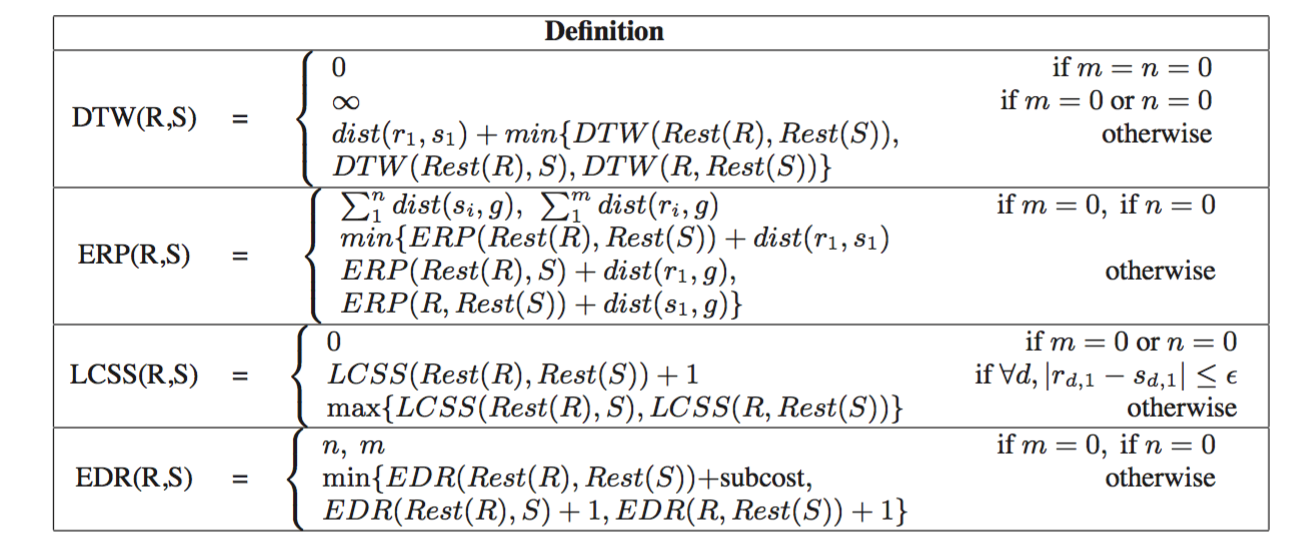
\includegraphics[width=1.0\textwidth]{chapter02/definition.png}
  \bicaption[fig:existing-sim-funs]{已有轨迹相似度函数定义}{已有轨迹相似度函数定义\footnotemark[1]}{Fig}{Definition of existing distance functions}
\end{figure}
\footnotetext[1]{$dist(ri,si)=$ L1 or L2 norm; $subcost = 0$ if $r1,t−s1,t$, else $subcost= 1$}

\section{相关实现技术介绍}
\label{sec:technology}

\subsection{Flask应用框架}
\label{subsec:flask}
Flask框架是基于Python语言的一个Web开发微型框架。Web框架是指用于简单实现高效编写Web应用的软件发开框架。在Python中已有的流行Web框架有Django、Pyramid等。简而言之,当用户在浏览器内输入一个待访问的网址时,会发送一个特请HTTP请求。与此同时,Web框架便负责来处理这个HTTP请求,并分配不同的访问地址到工作人员事先已经编写好的代码,生成HTML,最后创建附带内容的HTTP相应。

将Flask框架定义为Web微框架的原因是以为Flask本身只实现了Web应用中的核心内容。本质上,Flask只依赖两个外部库:提供代码模板的Jinja2模板和提供Web服务器网关接口、路由与调用的Werkzeurg WSGI工作集\cite{flasklibrary}。通过第三方库来完成表单处理、用户验证、数据库操作等等任务。

\subsection{Bootstrap}
\label{subsec:bootstrap}
Bootstrap是Twitter公司推出的一个用户Web前端的开源工具。作为目前最为主流的HTML/CSS和JS的开发框架,Bootstrap通常使用于响应式分布的Web项目只用。作为完全开源工具,Bootstrap中的预处理脚本可以为开发者提供可直接使用的CSS样式表;Bootstrap完成一种框架应用于全平台多种设备的高度移植性;Bootstrap提供全面的HTML元素、CSS组件和Javascript插件,且均具有文档说明。


%%%%%%%%%%


\subsection{大规模数据集群处理}
\label{subsec:bigdata-intro}
集群计算随着如今海量数据的发展在许多领域都有着广泛应用,以高效准确完成大量数据并行级的处理任务。集群计算需要提供本地化任务规划、高容错机制和数据负载平衡基本功能。除此之外,集群计算中我们也会关注某一个数据集运用在并行操作去完成指定目标任务。\emph{MapReduce}\cite{dean2008mapreduce}是目前分布式处理或并行计算常用的大规模数据处理和生成的编程模型。其工作的大致思路在于用户自定义合适的$map$函数去处理初步输入的键值对数据并产生中间键值对结果,之后定义$reduce$函数将中间结果以相同的关键字进行合并生成最终的结果。

对于数据密集型的应用而言,可扩展的分布式系统对于系统运行和数据处理都有着很重要的帮助。合理的分布式系统可以为系统提供在通用硬件上运行时的容错保护,并且能保证多用户请求的高度并行处理。\emph{Hadoop}分布式文件系统(\emph{HDFS})借鉴了\emph{Google}文件系统(\emph{GFS})的大部分设计架构并实现了高度的容错保护机制并且能良好地运行于廉价的硬件设备之上。与此同时,HDFS也保证了在应用中数据的高度吞吐速率,使得HDFS能高效运行具有很大数据集的任务或应用。

\subsubsection{Spark处理引擎简介}
\label{subsubsec:spark}
\emph{MapReduce}变成模型和\emph{HDFS}可在大规模数据密集型应用良好,但对于一些需要重复使用中间数据或需要暂时保留中间数据的应用处理中,之前常用的集群计算模型\emph{Hadoop}由于需要将中间数据读写与\emph{HDFS}中从而产生了中间读写时间浪费,从而影响了应用性能。基于这一点,\emph{Spark}\cite{zaharia2010spark}作为在主流针对大规模数据处理的集群计算模型之一,在保证之前集群计算模型功能的同时,使用一种名为弹性分布式数据集(\emph{Resilient Distributed Datasets})的抽象,使得其可以将集群任务中的中间结果保存于设备的内存之中,以便之后的读写操作。因此,在大数据挖掘领域中,\emph{Spark}能够比\emph{Hadoop MapReduce}能为高效的处理需要迭代数据的集群计算。

\subsubsection{弹性分布数据集RDD}
\label{subsubsec:rdd}
\emph{Spark}集群计算处理引擎与之前集群处理的主要不同点即在于其引入的弹性分布式数据集(\emph{RDD})这一抽象概念。这一分布式内存抽象使得用户或程序员可以在容错机制的保护下在大规模集群设备中运行基于内存的数据操作。\emph{RDD}高效处理大数据在应用中的重用问题,作为一个并行的数据结构可以方便用户在内存中处理集群计算的中间过程数据,因地制宜分割数据集以更合理将任务分配个对应的工作节点,再结合丰富的内定操作函数以快速处理数据。
而\emph{RDD}提供的生成模式也能为我们设计算法提供更多思路。\emph{RDD}可以通过$parallelize$函数将程序中已有的数据用于生成为\emph{RDD},或通过对例如\emph{HDFS}、\emph{Hbase}等等的外部文件系统或外部数据源来生成\emph{RDD}。

\subsubsection{Spark Standalone集群模式}
\label{subsubsec:standalone}
\emph{Spark}应用在集群模式运营中运行独立的进程组,通过驱动程序中的\emph{Spark}上下文变量\emph{SparkContext}来设定运行参数和初始化。运行过程主要根据\emph{SparkContext}来连接如图\ref{fig:clustermanager}\cite{sparkclustermanager}中具体不同种类的集群管理类型,并通过内定的\emph{Cluster Manager}来分配应用的资源获取。初始化成功后,\emph{Spark}通过获取集群节点上的执行进程并准备开始执行操作和处理数据。之后,\emph{Spark}会将应用代码分发给各个节点并使之运行。

\begin{figure}[!htp]
  \centering
  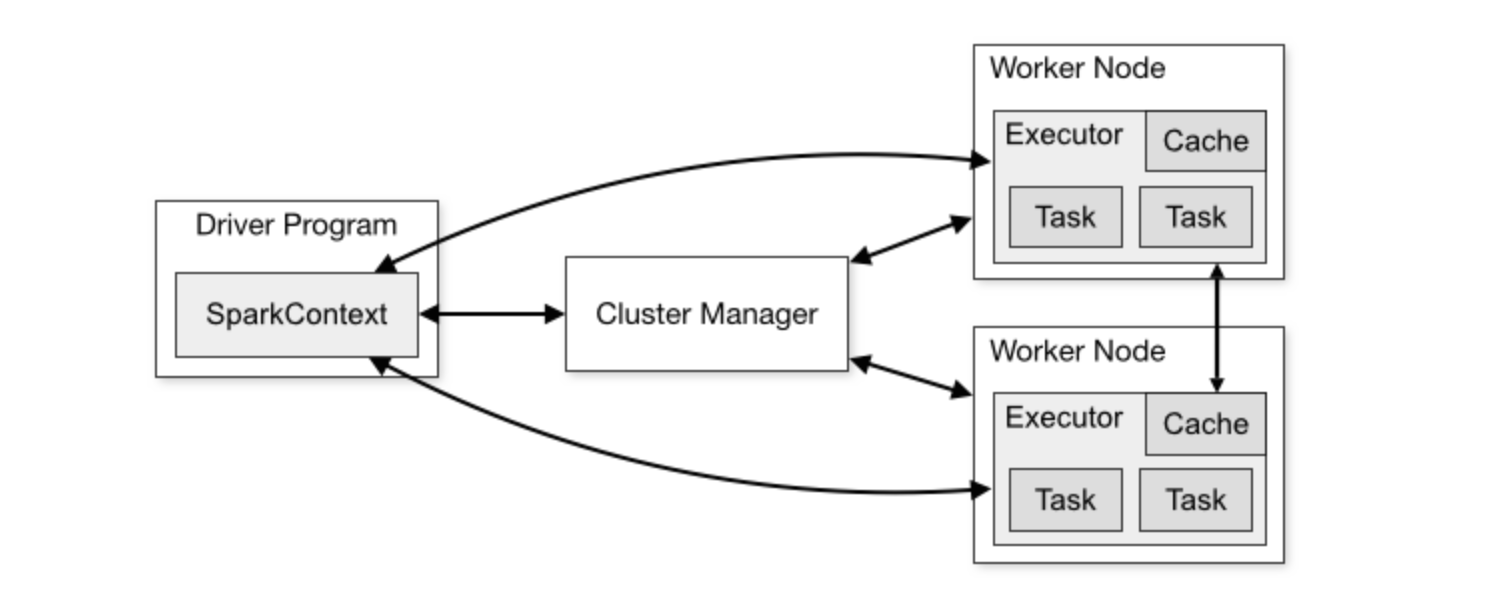
\includegraphics[width=1\textwidth]{chapter04/clustermanager.png}
  \bicaption[fig:clustermanager]{集群管理大致模式}{集群管理大致模式\cite{sparkclustermanager}}{Fig}{Cluster Managing Mode}
\end{figure}

在相似轨迹获取这一应用中,根据我们的应用场景和硬件设置,我们采用\emph{Spark}自带的\emph{Standalone}集群模式,其大致设计框架如图\ref{fig:standalone}\cite{hongzhi2017parallel}所示。

\begin{figure}[!htp]
  \centering
  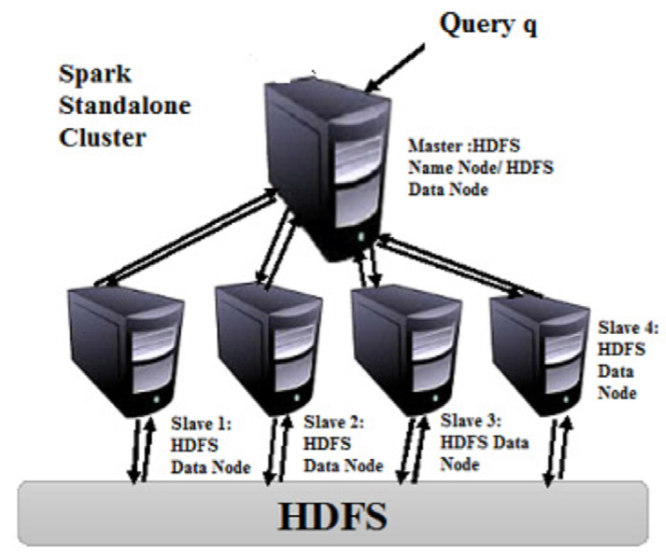
\includegraphics[width=0.5\textwidth]{chapter04/standalone.png}
  \bicaption[fig:standalone]{Spark Standalone集群结构}{Spark Standalone集群结构\cite{hongzhi2017parallel}}{Fig}{Spark Standalone Architecture}
\end{figure}

在\emph{Standalone}集群模式中,我们通过一个在\emph{Spark}分布式环境下的简要集群管理者来简单建立集群处理环境。在这一集群环境中,主节点(\emph{Master Node})为驱动程序运行的设备节点。驱动程序不仅是与用户交互信息的接口(\emph{interface})程序,也负责分布式运行在\emph{Spark}环境中进程的运行情况。子节点们(\emph{Slave Nodes})为启动在工作节点中的进程提供运行环境,这些进程运行任务代码并在内存或磁盘中储存数据。在相似轨迹搜索中,我们将轨迹数据和预处理好的轨迹索引R树结构存储在\emph{HDFS}上,集群环境中的工作节点可以通过设定好的参数无需秘钥的共享\emph{HDFS}上已存储好的数据,这样,我们可以将相似轨迹搜索任务进一步以分布式的方法进行处理。

%\section{相似度方程定义}
%\label{sec:similarityfunc}
%相似轨迹查询工作在某种意思上和时序数据相似查询共享一些方法定义。相似轨迹查询的首要步骤通过某种选定轨迹与轨迹点间的距离度量来定义相似度(或称为距离)方程,之后是设计高效的查询过程算法来解决从大规模数据库中找到符合要求的备选轨迹。定义相似度方法在过去有许多深度的讨论,之前的工作有通过利用离散傅里叶变化(Discrete Fourier Transform)[Ref bylocation2]将轨迹数据转化为多维空间上的点,任何通过比较这些点在特征空间上的欧式距离来比较轨迹数据时间的相似性。之后有科研人员在此工作成果的基础上通过改善实现子轨迹的匹配查询,并验证了离散小波变换(Discrete Wavelet Transform)的可行性。切比雪夫多项式(Chebyshev polynomials)在轨迹近似和索引方面有被证明是可应用的。但是这些方法的前提调前是需要轨迹上时序上具有相同的长度,因此这些转变返程所提供的相似度方法不适用与本文所提出的相似轨迹查询。

%\begin{figure}[!htp]
%  \centering
%  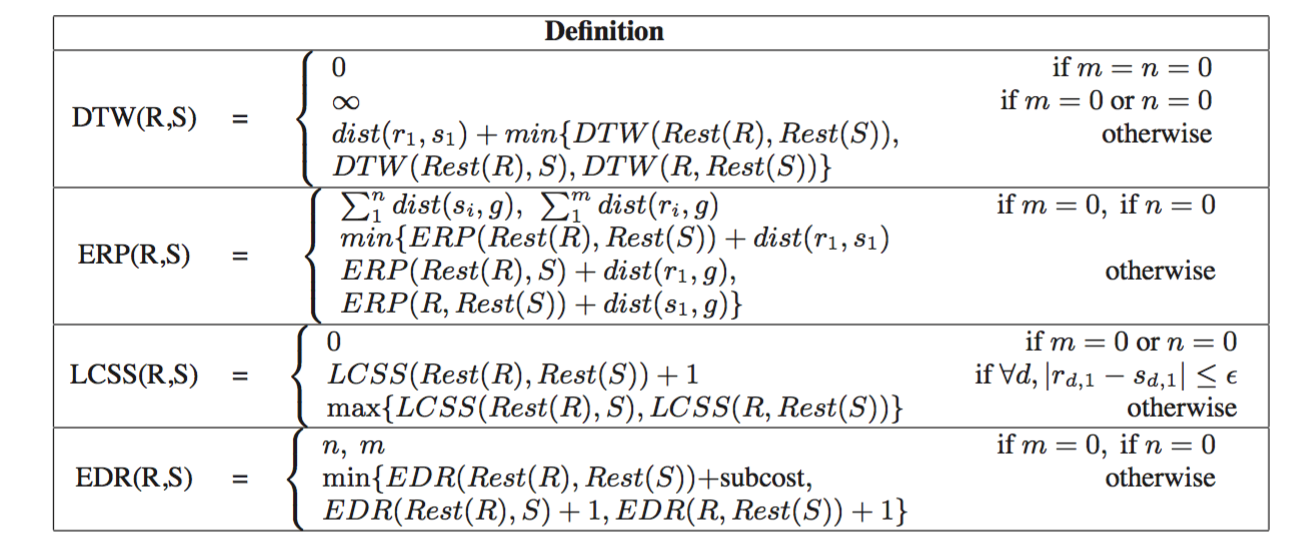
\includegraphics[width=1.0\textwidth]{chapter02/definition.png}
%  \bicaption[fig:2-1]{已有轨迹相似度函数定义}{已有轨迹相似度函数定义\footnotemark[1]}{Fig}{Definition of existing distance functions}
%\end{figure}
%\footnotetext[1]{$dist(ri,si)=$ L1 or L2 norm; $subcost = 0$ if $r1,t−s1,t$, else $subcost= 1$}

%图\ref{fig:2-1}是典型且常用的相似度方程定义。这些方程根据自身特点与优势应用于不同的场景中,包括欧氏距离方程(Euclidean Distance),动态时间规整(Dynamic Time Warping),最长公共子序列算法(Longest Common Subsequence),基于编辑代价的方法(Edit Distance With Real Penalty)和基于序列编辑的距离方法 (Edit Distance on Real Sequences)。动态时间规整(DTW)方法在比较轨迹之间相似性的过程中采用了时间偏移(time-shifting)来使得轨迹中的一些点可以尽可能多地重复出现以实现最好效果的校准。但这种方法在原有轨迹数据点出现误差(或称为噪声点)的时候会影响比较的准确性因为所有的点都需要被匹配。相比如动态时间规整方法(DTW),最长公共子序列(LCSS)选择忽略某些点以避免对他们的重排序过程,从结果上而言这种方法舍弃了偏离采样的误差点以提高了准确性,但需要人为预定距离阈值以判断什么数据属于误差点。基于编辑代价的距离方法(EDR)与LCSS方法类似,他们最初提出是为了解决字符串匹配问题,在轨迹数据匹配这一方面他们均采用一个阈值参数来判断两个点是否匹配,但EDR考虑了距离之间的衡量代价以决定是否将两个点进行匹配。在此基础上基于序列编辑的距离方法(ERP)结合EDR和DTW方法选择固定点进行距离计算。

%相似度方法通常根据具体的应用进行具体的选取。但上述的相似度方法主要是基于轨迹与轨迹之前相似度的查询,在本文设计的相似轨迹查询方法上的应用度并不理想,本工作的查询条件是基于一组地理坐标点的查询,并且工作更关注与一条轨迹是否能够很好地连接上给定的一组查询点,从而提供基于轨迹点的相似轨迹结果。因此,在这样的情景下,我们需要定义一个新的相似度方程。


%%%%%%%%%%

\subsection{轨迹数据预处理}
\label{subsec:preprocess}

\subsubsection{WGS84坐标系统转换至GCJ-02坐标系统}
\label{subsubsec:coord-transform}
WGS84(World Geodetic System1984)坐标系统是GPS数据所基于的坐标系统,这一坐标系是通过世界卫星观测站所检测到的地理坐标。这一坐标系并不能直接应用在中国国家的地图坐标显示中,因为中国国家会测局在地理信息系统中使用的是基于GCJ-02的坐标系统,这一坐标系统也称为火星坐标系统。如果直接将WGS84坐标数据应用于使用GCJ-02的地图显示接口,则会造成100米到700米范围内的显示误差。同理,用户使用GCJ-02地图点击获得的地理位置查询点也会在相似轨迹查询中因为与WGS84坐标系统的偏差因素造成查询结果的不准确性。在轨迹预处理最开始先将WGS84坐标数据根据已有的算法\footnotemark[1]参考转换成GCJ-02系统下的坐标
\footnotetext[1]{https://github.com/googollee/eviltransform}


\subsubsection{轨迹数据简化}
\label{subsubsec:trajectory simplification}
轨迹数据预处理中,轨迹数据的简化(或压缩)是比较重要一步。轨迹数据简化主要是指在保证轨迹的可利用性与大致准确的同时减少轨迹的点数目,以达到轨迹数据的传输、处理和存储上减少开销的目的。在本文的应用场景中,我们首先采用\emph{Douglas}–\emph{Peucker}算法\cite{visvalingam1990douglas}来完成我们的轨迹简化任务。该算法的主要思路在于将通过分而治之,将曲线轨迹表示成一系列点的方法,从而减少点的数目。如今GPS的数据采样通常较为频繁,因此在我们对轨迹处理的范围上来所,我们可以近似地将我们所运用的数据集中的轨迹看成是一条连续的曲线,通过\emph{Douglas}–\emph{Peucker}算法以及我们人为设定简化阈值,我们可以高效且合理地进行轨迹简化。

%\begin{algorithm}
% \begin{algorithm}[H] % 强制定位
%\caption{Douglas-Peucker算法}
%\label{algo:dp-ts}
%\begin{algorithmic}[1] %每行显示行号
%\Require 一条原始轨迹数据$Traj$, 简化阈值$\epsilon$ % 输入
%\Ensure 简化后的轨迹$Traj'$ % 输出
%\State $dis\_max \gets 0$;$index \gets 0$
%\For{$i = 1$ to $Traj.length-1$}
%	\State $temp\_dis \gets$ Traj[i]'s perpendicular Distance to Line(Traj[0], Traj[Traj.length])
%	\If{$temp\_dis > dis\_max$}
%		\State $dis\_max \gets temp\_dis$;$index \gets i$
%	\EndIf
%\EndFor
%\If{$dis\_max > \epsilon$}
%	\State half\_left $\gets Douglas$-$Peucker(Traj[0:index],\epsilon)$;
%	\State half\_right $\gets Douglas$-$Peucker(Traj[index:Traj.length],\epsilon)$;
%	\State $res \gets$ half\_left $\bigcup$ half\_right;
%	\Else
%	\State $res \gets \{Traj[0], Traj[Traj.length]\}$;
%\EndIf	
%\State \textbf{return} $res$;
%\end{algorithmic}
%\end{algorithm}

\emph{Douglas}–\emph{Peucker}算法首先连接轨迹首尾两点$Traj[0],Traj[Traj.length]$,遍历轨迹一遍得到离线段距离最大的点$Traj[index]$,计算该距离并与预先设定的阈值$\epsilon$比较。如果大于阈值$\epsilon$,则将轨迹以$Traj[index]$为中点分为两端,迭代重复上述工作;如果小于阈值$\epsilon$,则直接将线段段作为曲线的近似以做简化。当曲线完成上述任务,依次连接处理好的子线段,完成轨迹简化任务。

\subsection{轨迹数据索引与获取}
\label{subsec:index}
空间数据结构对从一个大规模轨迹数据集中获取特定轨迹数据是十分重要的。效率问题是查询大规模数据库或数据集来获取信息的首要考虑因素。而查询效率十分依赖于合理的轨迹索引。轨迹数据根据数据特点的不同姓对索引技术也有着特殊的要求。目前主流的索引技术主要有三类:1)基于空间维度的索引,利用R树(R-tree)索引进行查询。通过3DR树(3D R-tree)或者STR树(STR-tree)进行带有时间维度的查询;2)利用多版本的数据结构,根据特定情况使用 MR树(MR-tree)、HR树(HR-tree)、MV3R树(MV3R-tree)等等;3)将空间划分网格结构然后对应每个网格建立对应的空间索引,这类数据结构包括MTSB树(MTSB-tree)和SETI。本文中我们使用R树这一最基本的数据结构,其满足我们对算法的实现需求。

R树\cite{sellis1987r+,rtreedocument}数据结构在空间数据库中应用广泛,许多轨迹索引结构大体上是基于R树进行拓展。R树结构是一个平衡树结构,R树中的每一个节点代表包含其所有子节点一个区域,这个区域通常被称为最小区域箱(Minimum Bounding Box)。节点中的每一个数据体指向对应的子节点的最小区域箱信息。R树搜索的关键字是最小区域箱中的每一个节点。如图\ref{fig:2-2}\cite{sellis1987r+}所示的是R树数据结构的2种表现形式。在\ref{fig:2-2}(b)中我们看到树结构而图\ref{fig:2-2}(a)描述了数据和最小边界箱是如何分布在空间中的。
\\

\begin{figure}[!htp]
  \centering
  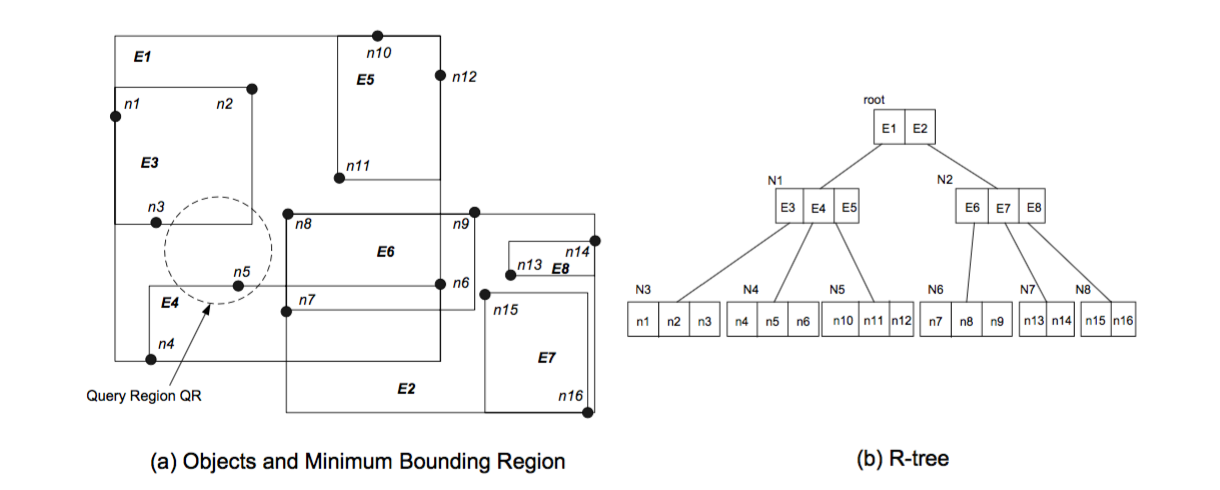
\includegraphics[width=1.0\textwidth]{chapter02/rtree.png}
  \bicaption[fig:2-2]{R树数据结构举例}{R树数据结构举例\cite{sellis1987r+}}{Fig}{Two views of an R-tree example}
\end{figure}

在图\ref{fig:2-2}中,根节点有两个数据体$E1$,$E2$,分别对应子节点$N1$,$N2$。$N1$代表的最小边界箱包含了其子节点$N3$、$N4$、$N5$以及数据体$E1$所具有的最小边界箱信息。值得注意的是空间点的体现只有在R树的叶节点上。R树可以应用在范围查询和近邻查询中。本文主要使用R树近邻查询这一属性。给定一个查询点,R树可以通过最优优先搜索(best-first)和深度优先搜索(depth-first)两种树遍历策略找到在数据集中最接近查询点的数据。在两种搜索策略中,查询点和每一个最小边界箱的距离被定义为变量$mindist$。之后的搜索过程基本遵从两种搜索策略各自算法。

在R树中插入一个新的节点大致需要以下几个步骤。当有新的轨迹数据需要被添加到已有的R树种,首先为待插入的轨迹数据点找到一个合适插入的子节点中。再寻找叶结点的过程中我们会选择符合最小边界范围且对R树扩展度最小的一个叶结点。然后若找到R树叶结点数据溢出,那么我们需要对叶子结点进行分裂操作;若没有溢出,则可以将待添加的轨迹数据加入到当前已经找到的叶子节点中。最后对R树进行变换向上传递并对树高进行增高以完成插入操作。删除操作近似于插入过程的逆过程,在此不予以赘述。

%%%%%%%%%%%%%%%%%%%%

\section{本章小结}
\label{sec:conclusion2}
本章节中,本文通过图标和伪代码讨论了相似轨迹查询方法的设计与实现的基本相关工作,对本文所应用的基本定义、处理思路和数据结构有了一个初步的了解。根据本文场景定义个性化的相似度方程后,我们在查询阶段需要通过多点输入的条件下进行归集查询。由于输入数据的轨迹点数目相对较少,我们可以借助已有的数据结构进行空间距离上搜索。利用R树和基于k最邻近的进行方法拓展是本文实现算法的基本思想,以快速的搜索并获取数据。根据上述本文工作相关工作描述,我们可以得出实现本文算法的先决条件目前都是基于只有已有的成熟工作。在下一章节中,本文将开始对相似轨迹查询方法进行理论讨论。